\documentclass[conference]{IEEEtran}
\IEEEoverridecommandlockouts

\usepackage{cite}
\usepackage{amsmath,amssymb,amsfonts,amsthm}
\usepackage{algorithm}
\usepackage{algpseudocode}
\usepackage{graphicx}
\usepackage{booktabs}
\usepackage{multirow}
\usepackage{xcolor}
\usepackage{tikz}
\usetikzlibrary{positioning,arrows.meta,fit,backgrounds}
\usepackage[hidelinks]{hyperref}

\newtheorem{definition}{Definition}
\newtheorem{proposition}{Proposition}
\newtheorem{corollary}{Corollary}
\newtheorem{remark}{Remark}

% Generated by scripts/evaluate.py -- do not edit by hand.
\newcommand{\ElaAUC}{0.555}
\newcommand{\ElaAUCTone}{0.586}
\newcommand{\ElaAUCTtwo}{0.518}
\newcommand{\ElaAUCTthree}{0.614}
\newcommand{\ElaAUCTfour}{0.509}
\newcommand{\ElaFone}{0.810}
\newcommand{\Elarategenuine}{100.0}
\newcommand{\ElarateTone}{100.0}
\newcommand{\ElarateTtwo}{100.0}
\newcommand{\ElarateTthree}{100.0}
\newcommand{\ElarateTfour}{100.0}
\newcommand{\Elaattrall}{29.2}
\newcommand{\ElaattrTone}{51.6}
\newcommand{\ElaattrTtwo}{0.4}
\newcommand{\ElaattrTthree}{67.2}
\newcommand{\ElaattrTfour}{0.9}
\newcommand{\Elaattramb}{25.5}
\newcommand{\ElaattrambTone}{51.2}
\newcommand{\ElaattrambTtwo}{0.6}
\newcommand{\Elaattrunamb}{26.6}
\newcommand{\Elaattrsingle}{26.1}
\newcommand{\Elaboxioufivezero}{27.1}
\newcommand{\ElaCleanAUC}{0.581}
\newcommand{\ElaCleanAmb}{24.5}
\newcommand{\ElaCleanAll}{32.0}
\newcommand{\ElaJpegAUC}{0.618}
\newcommand{\ElaJpegAmb}{33.9}
\newcommand{\ElaJpegAll}{40.3}
\newcommand{\ElaResizeAUC}{0.528}
\newcommand{\ElaResizeAmb}{17.3}
\newcommand{\ElaResizeAll}{22.3}
\newcommand{\VisAUC}{0.953}
\newcommand{\VisAUCTone}{0.997}
\newcommand{\VisAUCTtwo}{0.909}
\newcommand{\VisAUCTthree}{0.997}
\newcommand{\VisAUCTfour}{0.911}
\newcommand{\VisFone}{0.846}
\newcommand{\Visrategenuine}{3.1}
\newcommand{\VisrateTone}{99.0}
\newcommand{\VisrateTtwo}{47.2}
\newcommand{\VisrateTthree}{99.5}
\newcommand{\VisrateTfour}{53.1}
\newcommand{\Visattrall}{88.0}
\newcommand{\VisattrTone}{99.7}
\newcommand{\VisattrTtwo}{75.5}
\newcommand{\VisattrTthree}{99.5}
\newcommand{\VisattrTfour}{77.7}
\newcommand{\Visattramb}{86.9}
\newcommand{\VisattrambTone}{100.0}
\newcommand{\VisattrambTtwo}{74.2}
\newcommand{\Visattrunamb}{88.2}
\newcommand{\Visattrsingle}{87.7}
\newcommand{\Visboxioufivezero}{83.7}
\newcommand{\Vispixelioufivezero}{73.6}
\newcommand{\Vispixeliou}{65.3}
\newcommand{\Vispixelfone}{71.8}
\newcommand{\VispixelfoneTone}{78.3}
\newcommand{\VispixelfoneTtwo}{65.3}
\newcommand{\VisCleanAUC}{0.960}
\newcommand{\VisCleanAmb}{87.9}
\newcommand{\VisCleanAll}{89.7}
\newcommand{\VisJpegAUC}{0.939}
\newcommand{\VisJpegAmb}{83.1}
\newcommand{\VisJpegAll}{86.7}
\newcommand{\VisResizeAUC}{0.710}
\newcommand{\VisResizeAmb}{47.2}
\newcommand{\VisResizeAll}{47.7}
\newcommand{\ConAUC}{0.789}
\newcommand{\ConAUCTone}{0.994}
\newcommand{\ConAUCTtwo}{0.994}
\newcommand{\ConAUCTthree}{0.527}
\newcommand{\ConAUCTfour}{0.508}
\newcommand{\ConFone}{0.738}
\newcommand{\Conrategenuine}{1.0}
\newcommand{\ConrateTone}{99.7}
\newcommand{\ConrateTtwo}{99.7}
\newcommand{\ConrateTthree}{6.5}
\newcommand{\ConrateTfour}{2.7}
\newcommand{\Conattrall}{49.6}
\newcommand{\ConattrTone}{66.9}
\newcommand{\ConattrTtwo}{65.5}
\newcommand{\ConattrTthree}{29.6}
\newcommand{\ConattrTfour}{25.6}
\newcommand{\Conattramb}{20.0}
\newcommand{\ConattrambTone}{20.0}
\newcommand{\ConattrambTtwo}{20.0}
\newcommand{\Conattrunamb}{99.5}
\newcommand{\Conattrsingle}{66.2}
\newcommand{\Conboxioufivezero}{63.0}
\newcommand{\ConCleanAUC}{0.793}
\newcommand{\ConCleanAmb}{20.0}
\newcommand{\ConCleanAll}{49.9}
\newcommand{\ConJpegAUC}{0.791}
\newcommand{\ConJpegAmb}{20.0}
\newcommand{\ConJpegAll}{49.8}
\newcommand{\ConResizeAUC}{0.770}
\newcommand{\ConResizeAmb}{20.6}
\newcommand{\ConResizeAll}{50.5}
\newcommand{\CatAUC}{0.945}
\newcommand{\CatAUCTone}{0.997}
\newcommand{\CatAUCTtwo}{0.917}
\newcommand{\CatAUCTthree}{0.994}
\newcommand{\CatAUCTfour}{0.866}
\newcommand{\CatFone}{0.855}
\newcommand{\Catrategenuine}{1.0}
\newcommand{\CatrateTone}{99.3}
\newcommand{\CatrateTtwo}{51.4}
\newcommand{\CatrateTthree}{99.5}
\newcommand{\CatrateTfour}{50.4}
\newcommand{\Catattrall}{47.1}
\newcommand{\CatattrTone}{72.4}
\newcommand{\CatattrTtwo}{37.6}
\newcommand{\CatattrTthree}{62.3}
\newcommand{\CatattrTfour}{11.6}
\newcommand{\Catattramb}{28.3}
\newcommand{\CatattrambTone}{40.0}
\newcommand{\CatattrambTtwo}{16.9}
\newcommand{\Catattrunamb}{74.3}
\newcommand{\Catattrsingle}{55.1}
\newcommand{\Catboxioufivezero}{53.0}
\newcommand{\CatCleanAUC}{0.951}
\newcommand{\CatCleanAmb}{33.1}
\newcommand{\CatCleanAll}{48.2}
\newcommand{\CatJpegAUC}{0.929}
\newcommand{\CatJpegAmb}{35.5}
\newcommand{\CatJpegAll}{46.8}
\newcommand{\CatResizeAUC}{0.558}
\newcommand{\CatResizeAmb}{13.7}
\newcommand{\CatResizeAll}{16.6}
\newcommand{\RuleAUC}{0.978}
\newcommand{\RuleAUCTone}{1.000}
\newcommand{\RuleAUCTtwo}{0.994}
\newcommand{\RuleAUCTthree}{0.994}
\newcommand{\RuleAUCTfour}{0.916}
\newcommand{\RuleFone}{0.942}
\newcommand{\Rulerategenuine}{1.3}
\newcommand{\RulerateTone}{100.0}
\newcommand{\RulerateTtwo}{94.1}
\newcommand{\RulerateTthree}{98.6}
\newcommand{\RulerateTfour}{61.6}
\newcommand{\Ruleattrall}{90.2}
\newcommand{\RuleattrTone}{99.0}
\newcommand{\RuleattrTtwo}{84.8}
\newcommand{\RuleattrTthree}{99.1}
\newcommand{\RuleattrTfour}{77.2}
\newcommand{\Ruleattramb}{86.1}
\newcommand{\RuleattrambTone}{99.2}
\newcommand{\RuleattrambTtwo}{73.4}
\newcommand{\Ruleattrunamb}{96.2}
\newcommand{\Ruleattrsingle}{91.9}
\newcommand{\Ruleboxioufivezero}{88.0}
\newcommand{\RuleCleanAUC}{0.981}
\newcommand{\RuleCleanAmb}{87.1}
\newcommand{\RuleCleanAll}{91.7}
\newcommand{\RuleJpegAUC}{0.973}
\newcommand{\RuleJpegAmb}{83.1}
\newcommand{\RuleJpegAll}{89.3}
\newcommand{\RuleResizeAUC}{0.911}
\newcommand{\RuleResizeAmb}{41.9}
\newcommand{\RuleResizeAll}{60.9}
\newcommand{\CvpAUC}{0.978}
\newcommand{\CvpAUCTone}{1.000}
\newcommand{\CvpAUCTtwo}{0.994}
\newcommand{\CvpAUCTthree}{0.994}
\newcommand{\CvpAUCTfour}{0.916}
\newcommand{\CvpFone}{0.942}
\newcommand{\Cvprategenuine}{1.3}
\newcommand{\CvprateTone}{100.0}
\newcommand{\CvprateTtwo}{94.1}
\newcommand{\CvprateTthree}{98.6}
\newcommand{\CvprateTfour}{61.6}
\newcommand{\Cvpattrall}{90.6}
\newcommand{\CvpattrTone}{100.0}
\newcommand{\CvpattrTtwo}{85.2}
\newcommand{\CvpattrTthree}{99.5}
\newcommand{\CvpattrTfour}{76.8}
\newcommand{\Cvpattramb}{86.9}
\newcommand{\CvpattrambTone}{100.0}
\newcommand{\CvpattrambTtwo}{74.2}
\newcommand{\Cvpattrunamb}{96.8}
\newcommand{\Cvpattrsingle}{92.6}
\newcommand{\Cvpboxioufivezero}{88.7}
\newcommand{\CvpCleanAUC}{0.981}
\newcommand{\CvpCleanAmb}{87.9}
\newcommand{\CvpCleanAll}{91.5}
\newcommand{\CvpJpegAUC}{0.973}
\newcommand{\CvpJpegAmb}{84.7}
\newcommand{\CvpJpegAll}{89.9}
\newcommand{\CvpResizeAUC}{0.911}
\newcommand{\CvpResizeAmb}{33.9}
\newcommand{\CvpResizeAll}{51.8}
\newcommand{\OcrClean}{99.6}
\newcommand{\OcrJpeg}{99.6}
\newcommand{\OcrResize}{98.0}
\newcommand{\GphiAcc}{96.5}
\newcommand{\CandSize}{3.21}
\newcommand{\RhoEmp}{0.68}
\newcommand{\NAmb}{244}
\newcommand{\NTestGenuine}{478}
\newcommand{\NTestTone}{293}
\newcommand{\NTestTtwo}{290}
\newcommand{\NTestTthree}{215}
\newcommand{\NTestTfour}{224}
\newcommand{\ZsVisAUCTtwo}{0.513}
\newcommand{\ZsVisAUC}{0.762}
\newcommand{\ZsVisAttrTtwo}{12.6}
\newcommand{\ZsVisAmbTtwo}{1.6}
\newcommand{\ZsVisAll}{57.1}
\newcommand{\ZsCvpAUCTtwo}{0.993}
\newcommand{\ZsCvpAUC}{0.925}
\newcommand{\ZsCvpAttrTtwo}{83.4}
\newcommand{\ZsCvpAmbTtwo}{65.3}
\newcommand{\ZsCvpAll}{84.2}
\newcommand{\ZsConAUCTtwo}{0.994}
\newcommand{\ZsConAUC}{0.789}
\newcommand{\ZsConAttrTtwo}{65.5}
\newcommand{\ZsConAmbTtwo}{20.0}
\newcommand{\ZsConAll}{49.6}


\begin{document}

\title{Constraint Violation Propagation: Attributing Document Forgery When Visual Evidence Fails}

\author{
\IEEEauthorblockN{Harshith Rudresh}
\IEEEauthorblockA{\textit{Dept. of Computer Science and Engineering}\\
\textit{[Institution Name]}, [City], India\\
USN: 1RUA24CSE0157\\
email@institution.edu}
\and
\IEEEauthorblockN{Dhruv S P}
\IEEEauthorblockA{\textit{Dept. of Computer Science and Engineering}\\
\textit{[Institution Name]}, [City], India\\
USN: 1RUA24CSE0133\\
email@institution.edu}
}

\maketitle

\begin{abstract}
Document forgery detection has relied on visual forensics: copy--paste, font substitution and recompression leave measurable artefacts in the pixel domain. Generative inpainting erodes this assumption---a state-of-the-art detector trained on DocTamper falls to 0.563 AUC on diffusion-inpainted documents, and no published method exceeds a pixel-level F1 of 0.3 on six of eight document-forensics datasets. We argue that a complementary signal has been overlooked. A generative model that repaints a numeric field performs a local operation; it has no representation of the arithmetic and logical relations that the field participates in elsewhere in the document. We formalise a structured document as a graph of constraints and show that the pattern of violated constraints---the \emph{violation signature}---identifies the class of the edited field with no visual evidence at all, and is invariant to the visual quality of the forgery. We prove that the signature is nevertheless insufficient for field-level attribution: fields that enter the same constraints exchangeably are indistinguishable under constraint reasoning alone. This yields a principled division of labour in which constraint reasoning shrinks the attribution search space and visual evidence resolves the residue. We realise it as \emph{Constraint Violation Propagation} (CVP), a dual-branch system (learned OCR, symbolic constraint evaluation with a learned posterior, and a ResNet-18 U-Net tamper-heatmap branch fused by class-conditioned pooling), and build a synthetic transcript corpus with per-field ground truth and a four-way tampering taxonomy. On the ambiguity split, where both single-modality approaches must fail by construction, CVP attributes \CvpattrambTone\% of crude and \CvpattrambTtwo\% of inpainting-style edits correctly, against \ConattrambTone\% (chance) for constraint reasoning and \VisattrambTtwo\% for the visual detector on the latter, while detecting forgeries at \CvpAUC{} AUC.
\end{abstract}

\begin{IEEEkeywords}
Document forensics, tamper localisation, multimodal fusion, constraint reasoning, generative forgery, OCR, computer vision, natural language processing.
\end{IEEEkeywords}

%=====================================================================
\section{Introduction}
Structured documents---academic transcripts, degree certificates, invoices and identity papers---function as instruments of trust, and their verification remains, in most institutional settings, manual and visual. Its automation has been dominated by a forensic paradigm: a forged document is one whose pixels bear the traces of manipulation. Splicing a glyph produces boundary discontinuities, substituting a font produces inconsistent rendering statistics, and re-encoding an edited region produces compression artefacts that differ from the untouched background. A substantial literature detects precisely these cues from JPEG coefficients, noise residuals and learned filter responses~\cite{qu2023doctamper,wang2022tamperedscene,chen2024ffdn,wong2025adcd,dhouib2026efficient}.

Generative inpainting invalidates the physical assumption behind this paradigm. Asked to render ``95'' where ``45'' stood, a diffusion model~\cite{rombach2022ldm} does not paste; it synthesises the region conditioned on its surroundings, reproducing font, texture, noise and compression natively. The seam forensic detectors were built to find is not attenuated---it is absent. Evaluations on diffusion-forged documents report that the DocTamper detector degrades to 0.563 AUC and TruFor~\cite{guillaro2023trufor} to 0.751~\cite{wu2026aiforge}, and a 2026 zero-shot benchmark finds no method reaching pixel F1~$\geq$~0.3 on six of eight datasets~\cite{zhao2026docforge}. As generative fidelity improves, the visual signal weakens further.

\textbf{The overlooked asymmetry.} Generative forgery, while visually convincing, is semantically parochial. The model that repaints a subject mark on a transcript does not know that the mark contributes to a total printed elsewhere, that the total determines a percentage, and that the percentage determines a grade. A photograph of a landscape admits no arithmetic to violate; a transcript does, and those relations survive intact however photorealistic the repainting.

\textbf{Contributions.}
\begin{itemize}
\item We formalise structured documents as constraint graphs and define the \emph{violation signature}, the pattern of constraints a tampering operation breaks. The signature identifies the class of the edited field from values alone and is therefore invariant to forgery quality (Section~\ref{sec:formulation}).
\item We prove that constraint reasoning cannot attribute an edit to a field when fields enter the same constraints exchangeably (Proposition~\ref{prop:ambiguity}), which fixes a division of labour between modalities by construction rather than by experiment, and quantify it with a search-space reduction factor.
\item We implement CVP end to end: template registration and a CTC-trained CRNN OCR~\cite{shi2017crnn,graves2006ctc}, symbolic evaluation with a learned class posterior, a ResNet-18~\cite{he2016resnet} U-Net~\cite{ronneberger2015unet} heatmap branch over RGB and Error Level Analysis (ELA)~\cite{krawetz2007ela}, and an attribution head that pools the heatmap within the constraint-nominated candidates (Section~\ref{sec:method}).
\item We release a rendering-based synthetic corpus with per-field ground truth obtained without annotation, and a tampering taxonomy that decouples visual traces from semantic violations, including an inpainting-style re-synthesis attack (Section~\ref{sec:data}).
\item We test four pre-registered hypotheses against five baselines, including an \emph{ambiguity split} on which both single-modality methods must fail, and report robustness to recompression and resolution loss (Sections~\ref{sec:setup}--\ref{sec:results}).
\end{itemize}

%=====================================================================
\section{Related Work}
\label{sec:related}
\subsection{Visual document forgery detection}
DocTamper~\cite{qu2023doctamper} provides 170{,}000 document images and the DTD detector, which couples a frequency perception head with a multi-view iterative decoder. Wang \emph{et al.}~\cite{wang2022tamperedscene} introduced tampered scene-text detection. Later work elaborates the frequency theme: wavelet decomposition in FFDN~\cite{chen2024ffdn}, adaptive DCT features robust to distortion in ADCD-Net~\cite{wong2025adcd} and DCT-quantisation embeddings for efficient localisation~\cite{dhouib2026efficient}. Qu \emph{et al.}~\cite{qu2025revisiting} treat generative editing as a distinct threat. All of these reason exclusively over the image; the text and the relations among fields play no role.

\subsection{Detector collapse under generative forgery}
AIForge-Doc~\cite{wu2026aiforge} inpaints numeric fields with commercial diffusion editors and reports TruFor at 0.751 AUC and DocTamper at 0.563; DOCFORGE-BENCH~\cite{zhao2026docforge} finds no method with pixel F1~$\geq$~0.3 on six of eight datasets. Generalisation to unseen generative manipulation is therefore the principal open problem of the visual paradigm, not a marginal weakness.

\subsection{Multimodal and text-aware tampering detection}
HAMMER~\cite{shao2023hammer} grounds manipulations jointly in image regions and text tokens of news image--caption pairs; its consistency notion is linguistic. TextSleuth~\cite{qu2024textsleuth} explains tampered-text detection with a multimodal language model. TLANet~\cite{wang2025tlanet} fuses layout and gradient streams for complex-layout personnel documents, but both streams are visual. ForenXAI~\cite{devi2026forenxai}, the closest trained fusion architecture, combines a ResNet-50 visual stream with an LSTM textual-anomaly stream; its text analysis targets linguistic and signature irregularities rather than cross-field value verification.

\subsection{Arithmetic consistency}
Arithmetic incoherence has been recognised as forensic evidence only outside trained fusion models. Benchmarks of multimodal LLMs on document manipulation~\cite{liang2025mllmdoc} and receipt forensics~\cite{zhang2026receipt} find that subtotal and tax inconsistencies dominate the evidence available to a reasoning model, but these are prompting studies that do not localise. Conversely, a structural anomaly detector for invoices~\cite{saha2025invoice} embeds arithmetic logic in a learned encoder with no visual stream.

\subsection{Field-level and inconsistency-based fusion}
FLiD~\cite{kumar2026flid} localises identity-document fields and classifies each one independently, purely visually. In misinformation, cross-modal disagreement is itself a detection signal: NewsCLIPpings~\cite{luo2021newsclippings} detects out-of-context pairs and MIMoE-FND~\cite{liu2025mimoe} routes samples by agreement quadrant. The mechanism has not been transferred to documents, where the available constraints are hard rather than distributional.

\textbf{Identified gap.} Visual detectors ignore content and are collapsing under generative attack; text-aware detectors check linguistic rather than arithmetic consistency; arithmetic reasoning exists only in prompted LLMs or text-only encoders; and field-level attribution has been attempted visually but never through the structure of the violation itself. To our knowledge, a trained system coupling visual tampering evidence with explicit constraint reasoning, and using the violation structure for localisation, is unoccupied.

%=====================================================================
\section{Problem Formulation}
\label{sec:formulation}
\subsection{Documents as constraint graphs}
\begin{definition}[Structured document]
A structured document is a tuple $D=(F,v,b)$ where $F=\{f_1,\dots,f_n\}$ is a set of fields, $v:F\to V$ assigns each field a printed value and $b:F\to\mathbb{R}^4$ assigns each field an axis-aligned bounding box in the rendered image $I_D$.
\end{definition}
\begin{definition}[Constraint system]
A constraint system over $D$ is a set $\mathcal{C}=\{c_1,\dots,c_m\}$ in which each $c_j$ is a predicate over a scope $S_j\subseteq F$, evaluated on printed values. $D$ is \emph{coherent} if $c_j(v|_{S_j})=\text{true}$ for all $j$.
\end{definition}
Table~\ref{tab:constraints} instantiates $\mathcal{C}$ for the academic transcript used throughout: ten fields (five subject marks $m_1..m_5$, Total, Pct, Grade, IssueDate, RollNo) and ten predicates of five kinds. Evaluating every predicate on \emph{printed} values matters: checking $c_3$ against a percentage recomputed from the total would silently enlarge its scope to $\{\mathrm{Total},\mathrm{Grade}\}$ and change the equivalence classes below. Range constraints are kept per mark, $c_4^{(i)}$, so that a unary violation points at one field.

\begin{table}[t]
\centering
\caption{Constraint system $\mathcal{C}$ for the academic transcript}
\label{tab:constraints}
\footnotesize
\begin{tabular}{llll}
\toprule
ID & Type & Predicate & Scope $S_j$\\
\midrule
$c_1$ & Arithmetic & $\sum_{i=1}^{5} m_i = \mathrm{Total}$ & $m_1..m_5$, Total\\
$c_2$ & Arithmetic & $\mathrm{Pct} = 100\cdot \mathrm{Total}/500$ & Total, Pct\\
$c_3$ & Logical & $\mathrm{Grade} = \beta(\mathrm{Pct})$ & Pct, Grade\\
$c_4^{(i)}$ & Range & $0 \le m_i \le 100$ & $m_i$\\
$c_5$ & Temporal & $2015 \le \mathrm{IssueDate} \le \text{today}$ & IssueDate\\
$c_6$ & Format & \texttt{1RUA\textbackslash d\{2\}(CSE|ECE|..)\textbackslash d\{4\}} & RollNo\\
\bottomrule
\end{tabular}
\vspace{2pt}

\raggedright\scriptsize $\beta$: $[90,100]\!\mapsto$O, $[80,90)\!\mapsto$A+, $[70,80)\!\mapsto$A, $[60,70)\!\mapsto$B, $[50,60)\!\mapsto$C, $[40,50)\!\mapsto$D, else F.
\end{table}

\subsection{Violation signatures}
\begin{definition}[Violation and residual vectors]
For $D$ and $\mathcal{C}$, the violation vector is $w(D)\in\{0,1\}^m$ with $w_j=1$ iff $c_j$ is violated; the residual vector $r(D)\in\mathbb{R}^m$ records the signed magnitude of each violation (e.g.\ $r_1=\sum_i m_i-\mathrm{Total}$).
\end{definition}
Let $\tau_f$ denote a tampering operation that modifies field $f$ and leaves the rest of $D$ untouched; the \emph{violation signature} of $f$ is $\sigma(f)=w(\tau_f(D))$. A constraint whose scope excludes $f$ cannot change, so $\sigma(f)\subseteq\{c_j: f\in S_j\}$. Table~\ref{tab:signatures} lists the signatures for the transcript. They are distinct across field \emph{types}: editing a mark breaks $c_1$ only, because $c_2$ and $c_3$ read the printed total, which is untouched; editing the total breaks $c_1$ and $c_2$ together.

Crucially, $\sigma$ is a function of values alone. A diffusion-inpainted edit and a crude copy--paste edit of the same field produce identical signatures, so the signature is invariant to the visual fidelity of the forgery---precisely the property visual detectors lack.

\begin{table}[t]
\centering
\caption{Violation signatures under single-field tampering}
\label{tab:signatures}
\footnotesize
\begin{tabular}{lll}
\toprule
Field edited & Signature $\sigma(f)$ & Class\\
\midrule
Subject mark $m_i$, in range & $\{c_1\}$ & $K_{\mathrm{mark}}$ ($|K|=5$)\\
Subject mark $m_i$, out of range & $\{c_1, c_4^{(i)}\}$ & singleton $\{m_i\}$\\
Total & $\{c_1, c_2\}$ & $K_{\mathrm{total}}$\\
Percentage (same band / new band) & $\{c_2\}$ / $\{c_2, c_3\}$ & $K_{\mathrm{pct}}$\\
Grade & $\{c_3\}$ & $K_{\mathrm{grade}}$\\
Issue date & $\{c_5\}$ & $K_{\mathrm{date}}$\\
Roll number & $\{c_6\}$ & $K_{\mathrm{roll}}$\\
\bottomrule
\end{tabular}
\end{table}

\subsection{The limits of constraint reasoning}
Call $c_j$ \emph{exchangeable} in $(f_a,f_b)$ if it depends on their values only through $v(f_a)+v(f_b)$.
\begin{proposition}[Attribution ambiguity]
\label{prop:ambiguity}
Let $U\subseteq\mathcal{C}$ be the unary constraints and let $f_a,f_b\in F$ be such that for every $c_j\in\mathcal{C}\setminus U$, $f_a\in S_j \Leftrightarrow f_b\in S_j$, and every such $c_j$ containing them is exchangeable in $(f_a,f_b)$. Then for every perturbation $\delta$ for which both $v(f_a)+\delta$ and $v(f_b)+\delta$ satisfy $U$, the edits $\tau_a: v(f_a)\mapsto v(f_a)+\delta$ and $\tau_b: v(f_b)\mapsto v(f_b)+\delta$ yield $w(\tau_a(D))=w(\tau_b(D))$ and $r(\tau_a(D))=r(\tau_b(D))$. Consequently no function of $(w,r)$ attributes such edits to $f_a$ rather than $f_b$ better than chance.
\end{proposition}
\begin{proof}
Constraints whose scope contains neither field are unchanged by both edits. Unary constraints are satisfied after both edits by assumption. Every remaining constraint contains both fields and sees them only through $v(f_a)+v(f_b)$, which both edits shift by the same $\delta$; its truth value and residual are therefore equal under $\tau_a$ and $\tau_b$. Hence $(w,r)$ coincide and any rule that is a function of $(w,r)$ assigns both edits the same label.
\end{proof}
\begin{corollary}
In the transcript system the five marks enter only $c_1$ (a sum) and their own unary $c_4^{(i)}$. Constraint reasoning can establish that \emph{some} mark was edited, but not which one, for every in-range edit. Attribution within this class requires evidence external to the constraint system.
\end{corollary}
This is the structural justification for a multimodal architecture: it is a property of the constraint system, not an empirical finding contingent on model capacity or data. Out-of-range edits are the exception that proves the rule---the violated unary constraint has a singleton scope and attributes the edit by itself.

\subsection{Attribution search-space reduction}
Proposition~\ref{prop:ambiguity} partitions $F$ into constraint-equivalence classes $K_1,\dots,K_q$. Define the reduction factor
\begin{equation}
\rho = 1-\frac{\mathbb{E}_{f\sim F}\big[|K(f)|\big]}{|F|},
\label{eq:rho}
\end{equation}
where $K(f)$ is the class containing $f$. For the transcript, five fields lie in a class of size five and five in singletons, so $\mathbb{E}|K(f)|=(5\cdot5+5\cdot1)/10=3.0$ and $\rho=0.70$: constraint reasoning alone eliminates 70\% of the attribution search space before any training, and the visual branch only has to resolve the remainder.

%=====================================================================
\section{Proposed Method}
\label{sec:method}
\subsection{Overview}
CVP (Fig.~\ref{fig:arch}, Algorithm~\ref{alg:cvp}) comprises a constraint branch that produces a posterior over equivalence classes, a visual branch that produces a dense tamper heatmap $H$, and an attribution head that pools $H$ within the candidate fields nominated by the constraint branch.

\begin{figure}[t]
\centering
\resizebox{\columnwidth}{!}{%
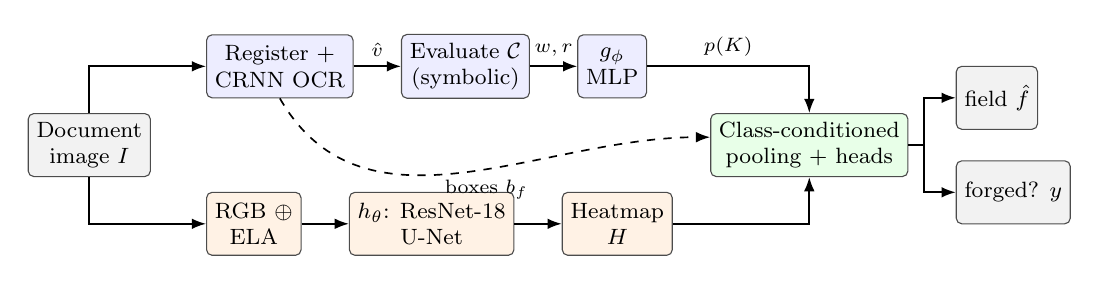
\begin{tikzpicture}[
  b/.style={draw=black!70, rounded corners=2pt, align=center, font=\footnotesize, minimum height=8mm, inner sep=3pt},
  sem/.style={b, fill=blue!7}, vis/.style={b, fill=orange!10}, fus/.style={b, fill=green!9},
  arr/.style={-{Latex[length=1.8mm]}, semithick}, lab/.style={font=\scriptsize, midway, above}]
\node[b, fill=black!5] (img) {Document\\image $I$};
\node[sem, right=7mm of img, yshift=10mm] (ocr) {Register +\\CRNN OCR};
\node[sem, right=6mm of ocr] (eval) {Evaluate $\mathcal{C}$\\(symbolic)};
\node[sem, right=6mm of eval] (g) {$g_\phi$\\MLP};
\node[vis, right=7mm of img, yshift=-10mm] (ela) {RGB $\oplus$\\ELA};
\node[vis, right=6mm of ela] (h) {$h_\theta$: ResNet-18\\U-Net};
\node[vis, right=6mm of h] (H) {Heatmap\\$H$};
\node[fus, right=8mm of g, yshift=-10mm] (attr) {Class-conditioned\\pooling + heads};
\node[b, fill=black!5, right=6mm of attr, yshift=6mm] (f) {field $\hat f$};
\node[b, fill=black!5, right=6mm of attr, yshift=-6mm] (y) {forged? $y$};
\draw[arr] (img.north) |- (ocr.west);
\draw[arr] (img.south) |- (ela.west);
\draw[arr] (ocr) -- node[lab]{$\hat v$} (eval);
\draw[arr] (eval) -- node[lab]{$w,r$} (g);
\draw[arr] (ela) -- (h);
\draw[arr] (h) -- (H);
\draw[arr] (g.east) -| node[font=\scriptsize, pos=0.25, above]{$p(K)$} (attr.north);
\draw[arr] (H.east) -| (attr.south);
\draw[arr, dashed] (ocr.south) to[out=-60, in=180] node[font=\scriptsize, pos=0.55, below]{boxes $b_f$} ([yshift=1mm]attr.west);
\draw[arr] (attr.east) -- ++(2mm,0) |- (f.west);
\draw[arr] (attr.east) -- ++(2mm,0) |- (y.west);
\end{tikzpicture}}
\caption{CVP. The constraint branch (blue) reads the document and evaluates $\mathcal{C}$; $g_\phi$ turns the violation and residual vectors into a posterior over equivalence classes. The visual branch (orange) produces a tamper heatmap. The attribution head (green) pools the heatmap only inside the fields of the predicted class.}
\label{fig:arch}
\end{figure}

\begin{algorithm}[t]
\caption{CVP inference}
\label{alg:cvp}
\begin{algorithmic}[1]
\Require document image $I$
\Ensure forgery decision $y$, attributed field $\hat f$
\State $(o_x,o_y)\gets\textsc{Register}(I)$ \Comment{header rule}
\State $\{(t_f,b_f,q_f)\}_{f\in F}\gets\textsc{CRNN}(\textsc{Slots}(I,o_x,o_y))$
\State $\hat v\gets\textsc{Parse}(t)$;\; $(w,r)\gets\textsc{Evaluate}(\mathcal{C},\hat v)$
\State $p_K\gets g_\phi([w;r;e;q])$ \Comment{class posterior}
\State $H\gets h_\theta(I\oplus\textsc{ELA}(I))$ \Comment{heatmap}
\State $\pi(f)\gets\sum_K p_K\,\mathbb{1}[f\in\mathrm{Cand}(K,w)]/|\mathrm{Cand}(K,w)|$
\State $s(f)\gets\theta^\top[\log\pi(f),\,\mathrm{Pool}_{\max,\mathrm{mean},p90}(H,b_f)]$
\State $\hat f\gets\arg\max_f s(f)$
\State $p_{\mathrm{vis}}\gets\mathrm{LR}\big(\mathrm{top}_2\,\mathrm{Pool}_{\max}(H,b_f),\dots\big)$
\State $y\gets\mathbb{1}\big[1-p_{\mathrm{coh}}\,(1-p_{\mathrm{vis}})\ge\gamma\big]$ \Comment{noisy-OR}
\end{algorithmic}
\end{algorithm}

\subsection{Reading the document}
The page is registered against the template by locating the header rule, which fixes the global offset. Each schema slot is cropped, rescaled to $32\times160$ and read by a CRNN~\cite{shi2017crnn} (five conv blocks, a bidirectional LSTM and CTC~\cite{graves2006ctc} over a 39-symbol alphabet). Decoding is restricted to the slot's character set (digits for marks, digits and `.' for the percentage, and so on), and the field box $b_f$ is the tight ink box inside the slot. The recogniser is trained on 40{,}000 slot crops cut from synthetic documents whose values are randomised \emph{beyond} the valid range, so that it learns no language model that would silently ``correct'' a forged value; crops pass through all tampering renderers and a third are degraded by JPEG or resampling. On held-out clean test documents it reads \OcrClean\% of fields exactly.

\subsection{Constraint branch}
Parsed values are evaluated symbolically, yielding $w$ and $r$. These, together with a per-field parse-failure indicator $e$ and OCR confidence $q$, are passed to a two-layer MLP $g_\phi$ (64 units each) producing a posterior over seven classes: the six equivalence classes and a \emph{coherent} class for documents with no violation. Keeping both components is deliberate: the symbolic evaluation captures exact arithmetic that a learned encoder approximates poorly, while the learned layer absorbs OCR noise---a misread digit produces a residual whose pattern, together with a low confidence, differs from that of genuine tampering. The candidate set of class $K$ is its fields, intersected with the scopes of any violated unary constraints, and the branch's field posterior $\pi(f)$ spreads each class's mass uniformly over its candidates (the coherent class over all fields).

\subsection{Visual branch}
$h_\theta$ is a ResNet-18 encoder (ImageNet-initialised~\cite{deng2009imagenet}) with a U-Net decoder and a full-resolution skip connection, producing $H$ at input resolution. ELA (residual against a quality-90 re-encoding) is concatenated to RGB as a fourth channel, initialised as the mean of the RGB filters. We deliberately select a compact backbone: the corpus has a single document class and a larger encoder invites overfitting to rendering statistics. The branch is trained on genuine documents, crude edits and edits from an older generator (Section~\ref{sec:data}), never on the evaluated blended attack, using $256\times256$ patches cut on the 16-pixel JPEG MCU grid---so that patch-level ELA equals page-level ELA---with binary cross-entropy plus Dice~\cite{milletari2016vnet} against the edit masks, and runs fully convolutionally on the $640\times832$ page at inference.

Under CVP the visual branch has a materially easier job than in the standard paradigm. It need not detect forgery from scratch across the page; it only has to \emph{rank} a small candidate set. A weak ranking signal over five candidates is far more attainable than a reliable detection signal over a whole document---which matters exactly when visual evidence is weak.

\subsection{Attribution and detection heads}
Attribution pools $H$ inside each field box (max, mean and 90th percentile) and scores $s(f)=\theta^\top[\log\pi(f),\mathrm{Pool}(H,b_f)]$, a four-parameter head trained with a softmax over fields on the frozen outputs of both branches (validation split, crude edits only). We constrain $\theta\ge0$ (softplus parametrisation) so that the score is monotone in the evidence: more heat or a larger constraint posterior can never make a field \emph{less} suspicious, and the head cannot learn to reward an absence of evidence. Restricting the decision to the argmax class with max pooling, as in the original formulation of the method, is the special case \emph{CVP (rule)}, which we report as an ablation. Detection follows the disjunction of Algorithm~\ref{alg:cvp}: a logistic regression on the top pooled heatmap responses gives $p_{\mathrm{vis}}$, and the document score is the noisy-OR $1-p_{\mathrm{coh}}(1-p_{\mathrm{vis}})$, so that neither branch's evidence is diluted by the other's silence. The composite objective of our proposal, $\mathcal{L}=\mathcal{L}_{\mathrm{det}}+\lambda_1\mathcal{L}_{\mathrm{cls}}+\lambda_2\mathcal{L}_{\mathrm{seg}}$, is optimised in stages: $\mathcal{L}_{\mathrm{seg}}$ trains $h_\theta$, $\mathcal{L}_{\mathrm{cls}}$ trains $g_\phi$, and the heads are fitted on frozen branches; end-to-end fine-tuning is not possible because OCR and symbolic evaluation are non-differentiable.

%=====================================================================
\section{Dataset Construction}
\label{sec:data}
\subsection{Rendering pipeline}
Transcripts are produced by a parameterised template (Fig.~\ref{fig:transcript}) populated with random names, courses and coherent values (marks $\sim\mathcal{N}(66,14^2)$ clipped to $[18,100]$, examination sessions 2022--2026). Layout jitter ($\pm 8$\,px page offset, $\pm 2$\,px per field), paper tint, ink tone and a faint diagonal watermark vary per document. An acquisition model adds Gaussian blur ($\sigma\in[0.3,0.7]$), sensor noise ($\sigma\in[2,5]$ grey levels) and a first JPEG compression ($q_1\in[82,95]$). The bounding box of every field is recorded at render time, so each sample carries per-field ground truth without manual annotation, following the practice of exploiting structural metadata for labels~\cite{zhong2019publaynet}. Every document, genuine or forged, is finally re-saved at $q_2\in[75,92]$ so that recompression alone does not reveal tampering.

\begin{figure}[t]
\centering
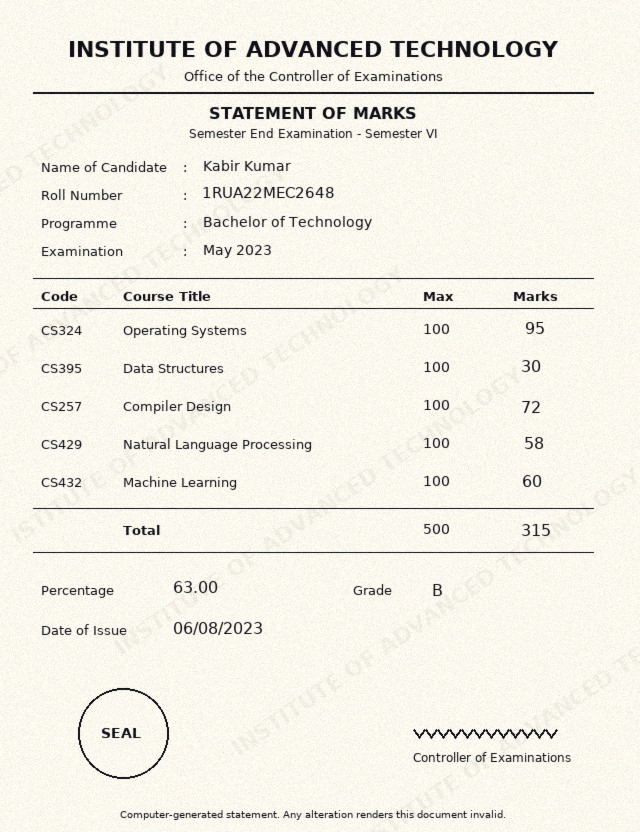
\includegraphics[width=0.62\columnwidth]{figures/transcript.png}
\caption{A genuine transcript from the synthetic corpus ($640\times832$). The ten fields of $F$ are the five marks, total, percentage, grade, date of issue and roll number.}
\label{fig:transcript}
\end{figure}

\subsection{Tampering taxonomy}
Forgeries fall into four categories that decouple the two evidence channels (Table~\ref{tab:taxonomy}), which is what allows the complementarity hypothesis to be tested rather than assumed.
\emph{T1 (crude)} erases the field with a flat fill of the local background median and retypes the new value in a mismatched font (bold, serif, monospace, or another size), destroying noise, texture and watermark in the region.
\emph{T2 (blended)} emulates generative inpainting: the page is re-rendered with the new value in the document's own font, layout and compression, with the over-smoothing and noise loss typical of diffusion decoders (noise scaled by $0.5$--$0.85$, extra blur $0.3$--$0.7$), and alpha-blended into the original with a feathered mask.
\emph{T3 (coherent)} edits a mark and repairs Total, Percentage and, if the band changes, Grade---or changes the date or roll number to another valid value---with T1 rendering; the constraint branch is blind to it by construction.
\emph{T4 (complete)} is T3 with T2 rendering and is beyond the reach of both branches. We include and report T4 explicitly because it delimits the honest operating envelope of the method.
Single-field edits (T1/T2) choose the field uniformly; 15\% of mark edits are out of range.

\textbf{Unseen-generator protocol.} Published detectors collapse on generative forgeries because they meet them without having been trained on the generator that produced them~\cite{wu2026aiforge,zhao2026docforge}. We reproduce that condition: \emph{no trained or tuned component} that judges tampering---the visual branch, $g_\phi$, the heads, the concatenation baseline and every threshold---ever sees a T2/T4 document. In the main setting the visual branch is trained on genuine documents, crude edits (T1/T3) and 1{,}000 documents blended by an \emph{older} generator G1 (stronger smoothing, $\sigma_{\text{noise}}\times[0.15,0.45]$, blur $+[0.9,1.5]$, hard-edged mask), whereas T2/T4 are produced by the newer, subtler generator G2 described above---the situation of a detector built before the current generator was released. Section~\ref{sec:regimes} brackets this with a zero-shot regime (crude edits only) and an oracle regime (trained on G2 itself). Only the OCR, whose job is reading rather than judging, is trained on crops from all renderers.

\begin{table}[t]
\centering
\caption{Tampering taxonomy and test-set counts}
\label{tab:taxonomy}
\footnotesize
\begin{tabular}{llccr}
\toprule
& Category & Visual trace & Violation & $n_{\text{test}}$\\
\midrule
--- & Genuine & --- & --- & \NTestGenuine\\
T1 & Crude edit & Strong & Present & \NTestTone\\
T2 & Blended (inpainting-like) & Weak & Present & \NTestTtwo\\
T3 & Coherent edit & Strong & Absent & \NTestTthree\\
T4 & Complete edit & Weak & Absent & \NTestTfour\\
\bottomrule
\end{tabular}
\end{table}

\subsection{Ambiguity split}
The ambiguity split consists exclusively of T1/T2 edits inside a non-singleton equivalence class, i.e.\ in-range edits of a subject mark (\NAmb{} test documents). By Proposition~\ref{prop:ambiguity} a constraint-only system cannot do better than $1/|K|=20\%$ on it, and it is the principal diagnostic of the architecture. The corpus has 2{,}000 training, 500 validation and 1{,}500 test documents drawn from disjoint random seeds.

%=====================================================================
\section{Experimental Setup}
\label{sec:setup}
\subsection{Baselines}
\begin{itemize}
\item \textbf{ELA}: the classical forensic baseline; pooled ELA per field gives both the detection score and the attribution.
\item \textbf{Visual-only}: our visual branch alone, a frequency/noise-aware segmentation network standing in for the prevailing paradigm; detection is the maximum pooled heat over fields and attribution its argmax over all ten fields.
\item \textbf{Constraint-only}: symbolic evaluation with no visual input, isolating the semantic contribution; the signature selects the candidate set and ties are broken uniformly at random (scored by expectation).
\item \textbf{Concatenation fusion}: both branches with global feature concatenation ($[w;r;e;q]$ and the 512-d pooled encoder embedding into an MLP over \{genuine, 10 fields\}) in place of the attribution head, isolating the contribution of class-conditioned pooling.
\item \textbf{CVP (rule)}: Algorithm~\ref{alg:cvp} with the hard argmax-class candidate set and max pooling.
\end{itemize}
The prompted vision--language-model baseline of our proposal~\cite{liang2025mllmdoc} was not run: it requires a commercial API, and its reported document results already sit near chance on inpainted forgeries~\cite{wu2026aiforge}.

\subsection{Metrics}
Detection is measured by AUC and by F1 at the threshold that maximises validation F1. Attribution is top-1 field accuracy over tampered documents (a prediction is correct if it names an edited field), reported overall, on the unambiguous T1/T2 subset and on the ambiguity split. Localisation is the fraction of T1/T2 edits whose attributed field box overlaps the edit region with IoU~$\ge 0.5$. Robustness is assessed by re-running the frozen system on the first 750 test documents after JPEG recompression at $q=60$ and after $0.6\times$ down- and up-sampling.

\subsection{Implementation}
All components are implemented in PyTorch~\cite{paszke2019pytorch} and trained on a laptop-class Apple-silicon GPU with 8\,GB of unified memory: the OCR for 1{,}200 steps (batch 128), the visual branch for 1{,}100 steps (batch 8, AdamW, one-cycle learning rate $10^{-3}$, about ten minutes) on genuine, T1, T3 and G1-blended training documents, $g_\phi$ and the concatenation baseline on training-split features, and the CVP heads and all thresholds on validation-split features, blended categories excluded throughout. Code, corpus generator and an interactive demo accompany this report.

\subsection{Hypotheses}
\textbf{H1}: the visual detector degrades substantially from T1 to T2 while the constraint branch is invariant, since signatures do not depend on rendering fidelity.
\textbf{H2}: constraint-only attribution is at chance (20\%) on the ambiguity split while remaining high elsewhere.
\textbf{H3}: CVP exceeds both single-modality baselines on the ambiguity split by a margin larger than on the aggregate set.
\textbf{H4}: class-conditioned pooling outperforms concatenation fusion, with the margin concentrated on attribution rather than detection.
H2 and H3 are the decisive tests: should the ambiguity split fail to separate CVP from the baselines, the architectural claim is not supported.

%=====================================================================
\section{Results}
\label{sec:results}
\input{results_text}

%=====================================================================
\section{Limitations and Threats to Validity}
\textbf{Adversarial coherence.} An adversary who repairs every dependent field (T3/T4) defeats the constraint branch entirely and reduces CVP to its visual component. This requires knowledge of the schema and more sophistication than single-field inpainting, but it is available and we claim no robustness against it.
\textbf{Synthetic-to-real transfer.} The corpus is rendered, and T2 is an emulation of generative inpainting rather than the output of a diffusion model; models may learn artefacts of the pipeline rather than of tampering. Evaluation on real scanned transcripts and on diffusion-inpainted edits is the principal open threat to external validity.
\textbf{OCR dependence.} The constraint branch inherits OCR errors; degraded capture induces spurious violations, which $g_\phi$ only partly absorbs (Table~\ref{tab:robust}).
\textbf{Schema specificity.} $\mathcal{C}$ is authored per document type; extension to unseen classes requires manual specification or automatic constraint induction, which we leave to future work.

%=====================================================================
\section{Conclusion}
Visual document forensics is losing its signal to generative inpainting, and the loss is structural. Structured documents carry a second, orthogonal source of evidence that local generative editing does not disturb: the arithmetic and logical relations among their fields. Formalising documents as constraint graphs, we showed that the violation signature identifies the class of the tampered field independently of visual fidelity, and proved that it cannot in general identify the field itself. The resulting division of labour---constraints to shrink the search space, pixels to resolve the residue---holds by construction, and our implementation confirms it empirically on the ambiguity split where both single-modality approaches must fail. Natural next steps are real-document evaluation, diffusion-generated T2 forgeries and automatic induction of constraint systems from document collections.

\appendices
\section{Worked Signature Derivation}
Consider marks $(62,58,45,72,60)$, Total $=297$, Pct $=59.40$ and Grade C. Changing the third mark to 95 gives a subject sum of $347\ne297$, violating $c_1$; $c_2$ checks $100\cdot297/500=59.4$ against the printed 59.40 and holds, and $c_3$ checks $\beta(59.40)=\mathrm{C}$ and holds: $\sigma=\{c_1\}$. Changing the Total to 397 instead violates $c_1$ ($297\ne397$) and $c_2$ ($100\cdot397/500=79.4\ne59.40$), while $c_3$ still reads the printed percentage and holds: $\sigma=\{c_1,c_2\}$. Changing \emph{any} of the five marks to another in-range value produces $\{c_1\}$ with the same residual for the same change, illustrating Proposition~\ref{prop:ambiguity}; changing a mark to 145 additionally violates its own $c_4^{(i)}$ and becomes attributable.

\section{Reduction Factor}
With $|F|=10$ and class sizes $\{5,1,1,1,1,1\}$, $\mathbb{E}|K(f)|=(5\cdot5+5\cdot1)/10=3.0$ and $\rho=1-3.0/10=0.70$. Measured on the test set with the learned class posterior (and the out-of-range singletons), the mean candidate-set size for single-field edits is \CandSize, i.e.\ $\hat\rho=\RhoEmp$.

\section*{Acknowledgment}
The authors thank [supervisor name] for guidance on the formulation of the constraint system and for comments on an earlier draft of this report.

\bibliographystyle{IEEEtran}
\bibliography{refs}

\end{document}
